\documentclass[12pt, a4paper]{article}

\usepackage[utf8x]{inputenc}
\usepackage[lithuanian]{babel}
\usepackage[L7x]{fontenc}
\usepackage{lmodern}
\usepackage{verbatim} 
\usepackage{tocloft}
\usepackage{url}
\usepackage{setspace}
\usepackage{caption}
\renewcommand{\cftsecleader}{\cftdotfill{\cftdotsep}}
\usepackage{parskip} 
\usepackage{graphicx}
\usepackage{fixltx2e} % šitas dėl \textsubscript{}
\usepackage{color} % spalvinsim tekstą
\parindent = 1cm

\usepackage{mathtools} % pades rašyti matematinius intarpus
\usepackage{titlesec}
\titlelabel{\thetitle.\quad} % Padeda tašką po skyriaus numerio
\usepackage{indentfirst} % atitraukta pirmoji eilute
\usepackage{longtable} % darysim didelias lenteles
\usepackage{algorithm}
\usepackage{algpseudocode}
\usepackage[top=2cm, bottom=2cm, left=3cm, right=1.5cm]{geometry}
\usepackage{changepage}
\usepackage{pdfpages} % su šitua paketu galima įkelti pdf kaip puslapius
\linespread{1.5}

\usepackage{hyperref}
\hypersetup{
    colorlinks,
    citecolor=black,
    filecolor=black,
    linkcolor=black,
    urlcolor=black
}
\usepackage[all]{hypcap}

\begin{document}

\begin{titlepage}

\begin{center}
VILNIAUS UNIVERSITETAS\\
MATEMATIKOS IR INORMATIKOS FAKULTETAS\\
PROGRAMŲ SISTEMŲ KATEDRA\\
\vspace{150pt}

\huge \textbf{Daugiamačių duomenų klasifikavimo analizė\\}
\vspace{20pt}
\large\textbf{Classification analysis of high-dimensional data\\}
\vspace{20pt}
\small Bakalauro darbas\\
\vspace{40pt}
\end{center} 


\begin{flushleft}
Atliko: \hspace{50pt} Dainius Jocas \hspace{105pt}\textsubscript{(para\v{s}as)}

\vspace{10pt}
Darbo vadovas: \hspace{12pt} Dr. Juozas Gordevičius \hspace{65pt}\textsubscript{(para\v{s}as)}

\vspace{10pt}
Darbo recenzentas: Dr. Vardenis Pavardenis \hspace{50pt}\textsubscript{(para\v{s}as)}
\\
\vspace{130pt}
\end{flushleft}

\begin{center}
VILNIUS - 2012
\end{center}

\end{titlepage}

\section*{SANTRAUKA}

Čia bus santrauka lietuvių kalba.
\newpage

\section*{SUMMARY}
\label{summary}

This bachelor thesis is dedicated to classification analysis of noisy, high-dimensional, small-sample biomedical data, which is often found in genetical, gene expression, epigenetics research. Next, we study feature selection methods as they are necessary for the analysis of high-dimensional data. We put special emphasis on robustness of feature selection because this is of paramount importance in the biomedical domain. We evaluate different feature selection methods with respect to computation complexity, accuracy of resulting classifier robustness of selected features. Experimental analysis revieled that there is no single best method for the given data and application domain. Therefore, in the summary of our work we provide directions for future research.

\textbf{Keywords:} high-dimensional data, machine learning, classification, feature selection, robustness of feature selection.

\newpage

\let \savenumberline \numberline
\def \numberline#1{\savenumberline{#1.}}
\setcounter{tocdepth}{5}
\setcounter{secnumdepth}{5}
\tableofcontents
\newpage

\addcontentsline{toc}{section}{{\c I}VADAS}
%% Įvade aprašomi darbo tikslai, nurodomas temos aktualumas, aptariamos teorinės darbo prielaidos bei metodika, apibrėžiamas tiriamasis objektas, apibūdinami su tema susiję literatūros ar kitokie šaltiniai, temos analizės tvarka, darbo atlikimo aplinkybės, pateikiama žinių apie naudojamus instrumentus (programas ir kt.). Darbo įvadas neturi būti dėstymo santrauka. Įvado apimtis 3–4 puslapiai.

\newpage
\section*{ĮVADAS}

%% JG: Idėja - naudok terminus "matai" ir "mėginiai". Kiekvienam mėginiui atliekama labai daug matavimų, iš to ir "daugiamatiškumas"

% JG: Paminėk, kad šiame darbe mes gilinamės į biomedicinoje kaupiamų genetinių duomenų analizės specifika. Šie duomenys ypatingi dėl daugiamatiškumo, mažo mėginių kiekio, triukšmingų matavimų.

Nuolat vystosi technologijos skirtos gauti biomedicininius duomenis, pvz. genomo sekvenavimas\cite{pettersson2009generations}, o tai reiškia, kad didėja gaunamų duomenų detalumas. Detalumas reiškia, kad daugėja biomedicininius duomenis abibūdinančių faktorių arba matų skaičius. Duomenys, kurių kiekvienas mėginys aprašomas dideliu skaičiumi matų, yra vadinami daugiamačiais duomenimis.

Šiame darbe yra nagrinėjama biomedicinoje kaupiamų genetinių daugiamačių duomenų analizės specifika. Šie duomenys yra specifiški tuo, kad jie įprastai turi šimtus kartų daugiau matų nei mėginių. Kadangi mėginio gavimo kaina yra aukšta, turimas mažas mėginių skaičius. Biomedicininių duomenų analizę apsunkina ir tai, kad matavimai, kuriais tie duomenys gaunami, yra triukšmingi. Triukšmas matavimo metu atsiranda dėl cheminių reakcijų netikslumo, tiriamo organizmo sudėtingumo. Kai duomenys yra triukšmingi ir didėja juos apibūdinančių matų skaičius, didėja tikimybė duomenyse bus rasta atsitiktinių priklausomybių. Tai yra pagrindinė priežastis, kodėl biomedicininių duomenų analizės procesas yra sudėtingas.

%% JG: Būdai neatsiranda, o vystosi technologija. Jie nėra tikslesni, bet detalesni, t.y. kiekvienam mėginiui atliekama daugiau matavimų. 

%% JG: Nors matavimų kiekis didėja, mėginio kaina išlieka gana aukšta. Todėl biomedicinos eksperimentuose gaunami duomenys ypatingi tuo, kad matų visados ženkliai daugiau nei mėginių.

Biomedicininių duomenų klasifikavimo užduotis yra atskirti sveikųjų pacientų mėginius nuo sergančiųjų. Klasifikavimu siekiama nustatyti, kurie matai, veikdami drauge, geriausiai paaiškina skirtumą tarp ligos paveiktų ir nepaveiktų mėginių. Labiausiai ligą paaiškinančių matų nustatymas galėtų palengvinti tiriamų ligų diagnozės ir gydymo metodų kūrimą. Klasifikavimu yra vadinamas duomenų analizės procesas, kurio metu yra sukonstruojama funkcija, atskirianti duomenis į grupes (arba klases) pagal jų matus \cite{fisher1936use}. Sukonstruotos funkcijos yra vadinamos klasifikatoriais, o jų konstravimo algoritmai -- klasifikavimo algoritmais. Klasifikatoriai paruošiami naudojant turimus mėginius -- treniravimosi duomenis -- ir informaciją apie jų būklę (sveikas ar sergantis). Klasifikatoriaus ruošimo procesas yra vadinamas apmokymu. Klasifikatoriai yra validuojami su testiniais duomenimis Klasifikatoriai naudojami nustatant naujų, dar nematytų, mėginių būklę.

Dėl ,,daugiamatiškumo prakeiksmo`` (angl. \textit{the curse of dimentionality}) didėjant matų kiekiui mėginiai pasidaro panašūs, todėl bandymas juos klasifikuoti tolygus spėliojimui \cite{bellman1966adaptive}. Biomedicininių duomenų kontekste galima daryti prielaidą, kad ne visi matai yra susiję su tiriama problema, pvz. gaubtinės žarnos vėžiu, dėl to, kad duomenys yra daugiamačiai. Paprastai nagrinėjamai problemai svarbus yra mažas, palyginus su visu, matų kiekis.  Todėl biomedicininių duomenų daugiamatiškumui sumažinti yra naudojami informatyviausių matų atrinkimo metodai \cite{guyon2003introduction} (angl. \textit{feature selection}). Pagal tai, kaip susiję su klasifikatoriumi, matų atrinkimo metodai skirstomi į tris kategorijas \cite{saeys2008robust}: filtruojantys (angl. \textit{filter}), prisitaikantys (angl. \textit{wrapper}) ir įterptiniai (angl. \textit{embedded}) metodai. Filtruojančiais metodais pirmiausia yra atrenkami informatyviausi matai, o tada apmokomas klasifikatorius. Prisitaikančiųjų 
metodų atveju, pirma, apmokomas klasifikatorius su visais matais, antra, parenkamas matų poaibis ir apmokomas klasifikatorius, tada po daugkartinio matų aibių įvertinimo pagal klasifikavimo rezultatus yra nusprendžiama, kuris matų poaibis yra labiausiai tinkamas klasifikavimui. Įterptinių metodų atveju matų atrinkimo procesas yra neatsiejamas nuo klasifikavimo proceso -- pats klasifikatorius įvertina matus.

Matų atrinkimas yra svarbi biomedicininių duomenų apdorojimo (angl. \textit{preprocessing}) etapo dalis. Naudojant matų atrinkimo metodus, galima kovoti su daugiamatiškumo prakeiksmu matų skaičių priartinant prie mėginių skaičiaus. Todėl svarbu yra pasirinkti geriausiai tinkančią matų atrinkimo strategiją. Kadangi ir pačių matų atrinkimo metodų veikimas priklauso nuo konkrečių duomenų, tai paties matų atrinkimo metodo pasirinkimas yra sudėtinga užduotis. 

Dirbant su biomediciniais duomenimis dažniausiai turime tik kelias dešimtis mėginių, todėl, norint geriau įvertinti klasifikatoriaus tikslumą, yra naudojami pakartotinio mėginių poaibio atrinkimo (angl. \textit{resampling}) metodai: kryžminio patikrinimo (angl. \textit{cross-validation}) arba įkelčių (angl. \textit{bootstrap\footnote{Terminas \textit{bootstrap} ,,įkelties`` prasme pradėtas naudoti dar Rudolfo Ericho Raspės knygoje ,,Barono Miunchauzeno nuotykiai``(1785), kurioje Baronas Minchauzenas užkėlė save ant arklio tempdamas į viršų savo batų raištelius (angl. \textit{bootstraps}).}}). Šių metodų naudojimas su duomenimis, kurių tikrasis pasiskirstymas nėra žinomas, padeda įvertinti klasifikavimo rezultatų variabilumą (angl. \textit{variance}) ir sisteminį nuokrypį (angl. \textit{bias}).

Naudojant kryžminio patikrinimo metodą, daug kartų sudaromos skirtingos treniravimosi ir testinės mėginių imtys. Taikant atskirą šio metodo variantą, kryžminį patikrinimą išbraukiant po vieną mėginį (angl. \textit{leave-one-out cross-validation}), iš treniravimosi imties išbraukiamas vienas mėginys ir apmokomas klasifikatorius, kuris klasifikuoja išbrauktąjį mėginį. Procesas tęsiamas tol, kol suklasifikuojami visi objektai. Kitais kryžminio patikrinimo metodo variantais iš treniravimosi mėginių yra išmetama po keletą mėginių. Pagal tai, kiek testinių mėginių klasifikatorius priskyrė klaidingai kategorijai, yra nustatoma vidutinė klaidingo klasifikavimo tikimybė. Šiuo metodu gauti įverčiai pasižymi dideliu klasifikavimo rezultatų variabilumu \cite{braga2004cross}.

Naudojant įkelčių metodą, iš $n$ dydžio mėginių aibės yra paimama tokio pačio dydžio atsitiktinių mėginių imtis su pasikartojimais, kuri vadinama įkelties treniravimosi imtimi. Į šią imtį nepaimti mėginiai yra priskiriami testavimo imčiai. Naudojant įkelties treniravimosi mėginių imtį yra apmokomas klasifikatorius, kuris klasifikuoja testavimo imtį. Procesą kartojant gaunama klaidingo klasifikavimo tikimybės įverčių imtis. Šios imties vidurkis yra klaidingo klasifikavimo tikimybės įvertis. Dažniausiai naudojamas ,“0.623 įkelčių`` (angl. \textit{0.623\footnote{0.623 yra tikimybė mėginiui būti įtrauktam į treniravimosi imtį.} bootstrap}) įverčiu. Šiuo metodu gautas klaidingo klasifikavimo tikimybės įverti pasižymi mažu klasisifikavimo rezultatų variabilumu \cite{michie1994machine}.

%% JG: Kodėl klasifikuojama? Norima nustatyti, kokie matai, veikdami drauge, geriausiai paaiškina skirtumą tarp ligos paveiktų ir sveikų mėginių.

%% JG: Kokios yra tradicinės klasifikavimo strategijos ir kodėl jos neveikia daugiamačių duomenų atveju? Skaičiavimo laikas nėra problema - Random forests veikia visai neblogai tokiais atvejais. Daugiamatiškumas veda prie the curse fo dimensionality.

% JG: sumažinus naudojamų matų kiekį, matų kiekis priartėja prie mėginių kiekio ir tokiu būdu apeinamas daugiamatiškumo prakeiksmo problema. Biomedicinos duomenų kontekste, galima daryti prielaidą, kad dauguma matų yra beprasmiai, pvz., tik kai kurie genai įtakoja ligą, todėl matų mažinimimas yra prasmingas. Taip pat, kuriant medicininius diagnostikos įrankius, naudojamų matų kiekis įtakoja įrankio kainą. Todėl pageidautina turėti kuo mažiau matų.

Kadangi biomedicininiuose duomenyse reikšmingų matų kiekis tiriamai problemai yra nedidelis, todėl tyrėjams norint geriau suprasti nagrinėjamus biomedicininius duomenis yra svarbu orientuotis į mažesnį matų poaibį, kuris yra svarbus nagrinėjamai problemai. Tokioje situacijoje tampa svarbu, kaip varijuoja atrenkamų matų aibė, kai matų atrinkimas vykdomas su vis kitu mėginių poaibiu. Matai, kurie keičiant mėginių, naudojamų matų atrinkime, poaibį yra vėl ir vėl atrenkami, yra vadinami stabiliais matais \cite{devijver1982pattern}. Parametras, parodantis kaip stabiliai yra atrenkami matai, yra vadinamas stabilumu \textit{(angl. robustness)}. Tačiau skirtingi matų atrinkimo metodai tiems patiems mėginiams gali atrinkti skirtingus matus. Taip pat, suskaidžius duomenis į persidengiančius poaibius ir atrinkus tą patį kiekį matų tuo pačiu metodu, gaunamas skirtingas matų poaibis. Matų aibės sumažinimas paspartina biomedicininių duomenų tyrimus -- tyrėjams reikia atlikinėti bandymus su mažesniu mėginių skaičiumi. 
Kuriant medicininius diagnostikos įrankius, naudojamų matų kiekis įtakoja įrankio kainą. Todėl stabilių matų atrinkimas dirbant su biomedicininiais duomenimis yra svarbus.

% JG: Žiūrėkim į stabilumą kaip į šalutinį matų atrinkimo efektą, kurį svarbu pažaboti. Stabilumas svarbus, nes, analizuojant duomenis norima ne tik nustatyti, koks būtų vidutinis klasifikatoriaus tikslumas, bet ir sukurti tą vidutinį klasifikatorių. Norint pastarąjį sukurti, reikia žinoti, kuriuos konkrečius matus naudoti. 

% JG: Šitam paragrafe suplaki daug svarbių dalykų į krūvą ir juos turėtum būti paaiškinęs jau anksčiau. Mėginių trūkumas nėra tavo sprendžiama problema. Tačiau, kuo mažiau duomenų, tuo nestabilesni atrenkami matai. 

%Taigi, dirbant su daugiamačiais duomenimis, reikia atsižvelgti į keletą kriterijų:
%\begin{enumerate}
% \item Klasifikavimo tikslumą;
% \item Matų atrinkimo stabilumą, atsižvelgiant į klasifikavimo rezultatus;
% \item Triukšmo lygį duomenyse;
% \item Skaičiavimo išteklių naudojimo racionalumą.
%\end{enumerate}
%Reikalavimas vienu metu atsižvelgti į keletą kriterijų užduotį daro sudėtinga. Klasifikuojant daugiamačius duomenis uždavinys yra surasti geriausius rezultatus duodančią strategiją, kuri geriausiai atsižvelgia į minėtus kriterijus.

%Darbo eksperimentinei daliai reikalingus skaičiavimo išteklius, suteikė VU MIF skaitmeninių tyrimų ir skaičiavimų centras \cite{mif2012stsc}. Eksperimentuose buvo naudojami laisvai internete prieinami biomedicininių duomenų rinkiniai (angl. \textit{datasets}). Biomedicininių duomenų apdorojimo algoritmų implementavimui buvo naudojama R \cite{r2012statistics} programavimo kalba. Eksperimentai atlikti profesinės praktikos MII metu.

Matų atrinkimo stabilumo problemą Yang ir Mao \cite{yang2011robust} siūlė spręsti reitinguojant matus remiantis keletos matų atrinkimo metodų rezultatais. Galutinis matų reitingo sąrašas gaunamas, kai po kiekvieno matų atrinkimo yra išmetama viena žemiausią reitingą turintis matas iš matų aibės, ir matų atrinkimas yra kartojamas tol, kol nebelieka matų. Tačiau matų atrinkimo metodų kiekis yra ribotas ir skirtingų metodų dažnai negalima vykdyti išskirstytų skaičiavimų aplinkoje. Tai riboja šio metodo pritaikomumą daugiamačių duomenų analizėje.

Matų atrinkimo stabilumo problemą siūlyta spręsti surandant matų grupių tankio centrus ir naudoti matus, kurie artimiausi tiems centrams \cite{yu2008stable}. Pasiūlytas grupių tankių algoritmas užtrunka $O(\lambda n^2m)$ laiko, kur $n$ yra matų kiekis, o $m$ - mėginių skaičius. Vėliau Loscalzo ir kt. pasiūlė mokymo duomenis skaidyti poaibiais ir kiekviename poaibyje ieškoti tankių grupių, o tada imti sprendimą balsavimo principu \cite{loscalzo2009consensus}. Nors šie metodai siūlo stabilų matų atrinkimą, tačiau šių metodų panaudojamumą daugiamačiuose duomenyse riboja skaičiavimo sudėtingumas.

Šiame bakalauriniame darbe remiantis Yang, Mao bei Loscalzo darbuose pateiktomis įžvalgomis, bus stengiamasi pasiūlyti tyrimų kryptis, kurios galėtų padėtų sukurti metodus, skirtus spręsti stabilių matų atrinkimo problemą. Idėja yra sugrupuoti matus pagal greitą klasterizacijos algoritmą, išrinkti reprezentatyviausius matus, transformuoti matų erdvę ir joje vykdyti matų atrinkimą remiantis keletu matų atrinkimo metodų.

Šio darbo tikslas yra išanalizuoti darbo su daugiamačiais duomenis ypatybes. Šiam darbui yra keliamos tokios užduotys:
\begin{enumerate}
 \item Susipažinti su naujausiais klasifikavimo ir matų atrinkimo metodais;
 \item Atlikti matų atrinkimo metodų palyginamuosius eksperimentus;
 \item Pasiūlyti kryptis, kaip dabartiniai metodai gali būti patobulinti ir paruošti naujųjų metodų prototipus.
\end{enumerate}

Tolimesnė bakalaurinio darbo struktūra yra tokia: skyriuje


\newpage

\section{MAŠININIO MOKYMOSI APŽVALGA}
\label{darbu_apzvalga}

Mašininis mokymasis (angl. \textit{machine learning}) yra dirbtinio intelekto šaka, kurios tyrėjai siekia įgalinti kompiuterius tobulinti savo elgseną (mokytis) empirinių duomenų atžvilgiu \cite{duda2001pattern}. Pagal tai, kokie yra turimi empiriniai duomenys, mašininis mokymasis yra skirstomas į mokymąsi su mokytoju (angl. \textit{supervised learning}) ir mokymąsi be mokytojo (angl. \textit{unsupervised learning}). Toliau šiame skyriuje apžvelgiami mašininio mokymosi pagrindai: mokymasis su mokytoju, mokymasis be mokytojo, atraminių vektorių klasifikatoriai, \textit{Random Forest} klasifikatorius.

\subsection{Mokymasis su mokytoju}

Žmonės mokosi iš patirties, tačiau, skirtingai nei žmonės, kompiuteriai patirties neturi, todėl kompiuteriai turi mokytis iš patyrimą apibūdinančių duomenų -- mokymosi duomenų (angl. \textit{training data}). Mokymosi su mokytoju tikslas yra sukonstruoti funkciją, kuri galėtų būti naudojama nuspėti testavimo duomenų (angl. \textit{testing data}) charakteristikų reikšmes pagal mokymosi duomenis. Šiame kontekste mokytoją reikia suprasti kaip išankstinį mokymosi duomenų spėjamų charakteristikų žinojimą. Kitaip tariant, mokymosi su mokytoju metodais yra sprendžiami uždaviniai, kuriems atsakymus galima patikrinti. Pagal tai, kokias charakteristikas bandoma nuspėti mokymasis su mokytoju yra skirstomas į dvi rūšis:
\begin{enumerate}
  \item Klasifikavimas (angl. \textit{classification}) -- pagal mokymosi duomenų nepriklausomus kintamuosius bandoma nuspėti kokybinius (kategorinės reikšmės) priklausomus kintamuosius.
  \item Regresinė analizė (angl. \textit{regression}) -- pagal mokymosi duomenų nepriklausomus kintamuosius bandoma nuspėti kiekybinius (tolydinės reikšmės) priklausomus kintamuosius.
\end{enumerate} 

%% JG: Pateik vizualų klasifikavimo pavyzdį iliustruojanti visus 3 etapus.
%% DJ: Vizualų, ta prasme su paveiksliukais ar ir tas pavyzdys su paštu pakankamai vaizdingas?
%% JG: Reikia kitaip struktūrizuoti šitą skyrių: 
% +Pradžioj pasakyk, kad yra klasifikavimas ir regresija ir po
%  sakinįÂ kiekvienam.
% +Tada aptark klasifikavimą ir pateik pavyzdį. 
% +Tada pateik regresijos pavyzdį.
% +Tada parašyk, kad šiame darbe studijuojama klasifikavimo problema.

\subsubsection{Klasifikavimas}

Mašinininio mokymosi kontekste klasifikavimu yra vadinama problema, kai pagal mokymosi duomenis reikia nustatyti, kuriai klasei priklauso objektas. Klasifikavimo procesas trimis etapais pavaizduoti ~\ref{fig:classification_process} pav. srautų diagramoje. Klasifikavimo etapai:
\begin{enumerate}
 \item Visa mokymosi duomenų aibė yra atsitiktinai padalinama į dvi nesikertančias aibes: treniravimos duomenys (pvz. 90\% visų mokymosi duomenų) ir testiniai duomenys(pvz. likę 10\%);
 \item Pagal turimus treniravimosi duomenis yra atrenkami informatyviausi matai, pvz. naudojant Relief metodą. Remiantis atrinktaisiais matais yra konstruojamas klasifikatorius - funkcija, pagal kurią nematyti mėginiai bus priskirti vienai iš klasių.
 \item Sukonstruotu klasifikatoriumi testiniai duomenys yra suskirstomi į klases. Pagal tai, kiek mėginių klasifikatorius priskyrė teisingoms klasėms yra vertinama klasifikatoriaus tikslumas. Klasifikatorius validuojamas naudojant tokius metodus kaip kryžminis patikrinimas (angl. \textit{cross validation})
\end{enumerate}

Dirbant su biomedicininiais duomenimis tipinė užduotis yra pagal paciento mėginį apibūdinančius matus sukonstruoti klasifikatorių, kuris bandys nuspėti, kuriai pacientų grupei -- sergančiųjų ar sveikųjų -- priklauso tiriamasis mėginys.
\begin{figure}
 \centering
 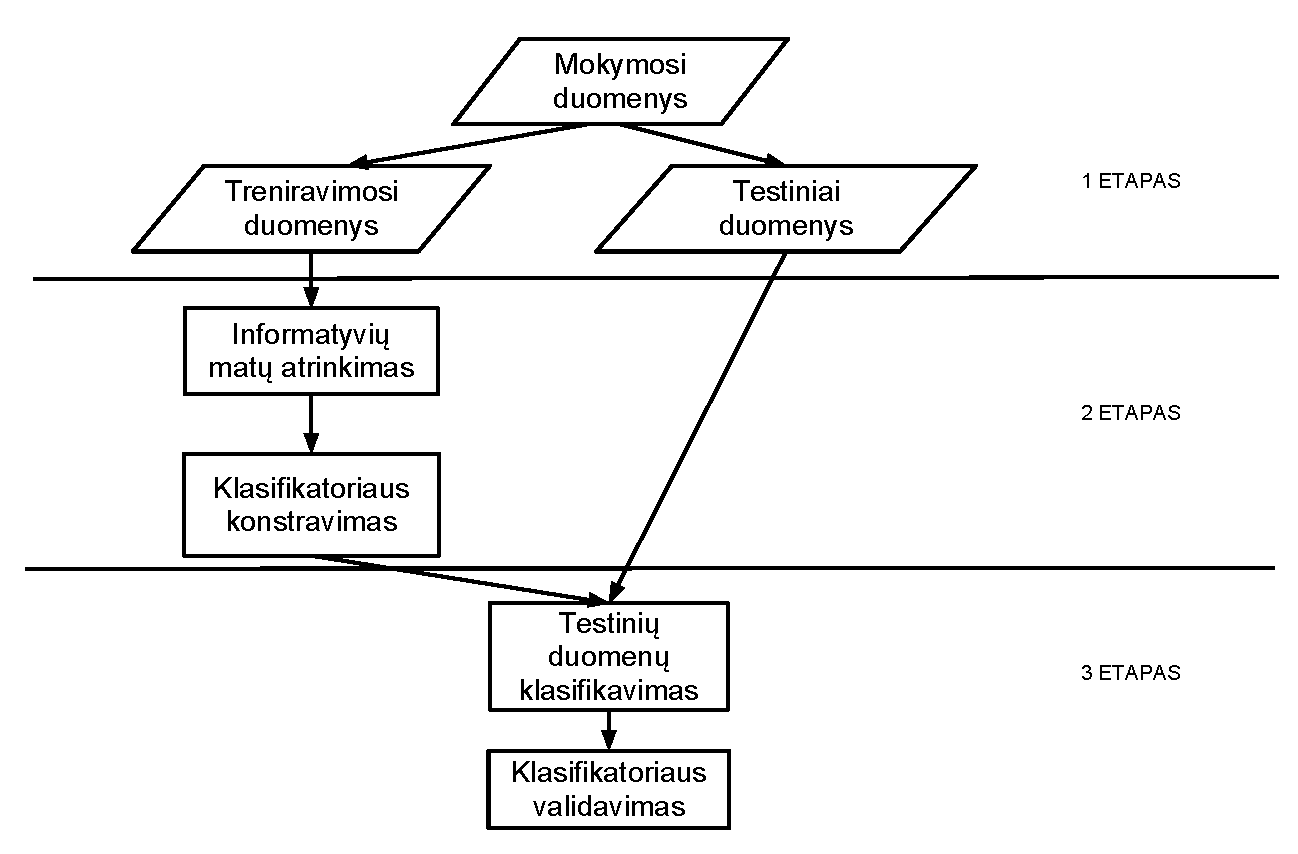
\includegraphics[width=\textwidth]{images/classification_process.pdf}
 \caption{Klasifikavimo srautų diagrama su paaiškinimais.}
 \label{fig:classification_process}
\end{figure}
Klasifikavimą galima vertinti pagal:
\begin{itemize}
 \item klasifikavimo tikslumą (angl. \textit{accuracy}) -- santykį tarp teisingai suklasifikuotų mėginių ir visų mėginių;
 \item klasifikavimo nuostolius (angl. \textit{error rate}) -- santykį tarp neteisingai suklasifikuotų mėginių ir visų mėginių;
 \item ROC (angl. \textit{receiver operating characteristic}, ROC) kreivę -- *****TODO***** abscisių ašyje tikimybės (angl. \textit{false positive}) įvykio, ordinačių ašyje (angl. \textit{true positive}) įvykio.
\end{itemize}

\subsubsection{Regresinė analizė}

Mašininio mokymosi kontekste regresine analize yra vadinama problema, kai pagal patirtį apibūdinančius duomenis reikia nustatyti kiekybines duomenų charakteristikas. Regresinė analizė naudoja standartinius statistinius metodus, tokius kaip mažiausių kvadratų metodas (angl. \textit{least squares}). Regresinė analizė dažniausiai naudojama įvertinti (ang. \textit{forecast}) ateities duomenų vertes bei interpoliacijai -- tikėtinos reikšmės tarp keletos taškų įvertinimui. 

Dirbant su biomedicininiais duomenimis regresinė analizė gali būti taikoma bandant nuspėti vėžio stadiją mėginiui. Tačiau regresinė analizė dirbant su biomedicininiais duomenimis yra naudojama rečiau negu klasifikavimas, todėl toliau šiame darbe bus nagrinėjama klasifikavimo problema.

\subsection{Mokymasis be mokytojo}

Mašininio mokymosi kontekste dažnai sutinkamas uždavinys yra į prasmingas grupes sugrupuoti turimus duomenis, kurių grupavimas iš anksto nėra žinomas. Tokie uždavinai yra sprendžiami mokymosi be mokytojo metodais. Mokymosi be mokytojo metodų pagrindinis principas -- maksimizuoti mėginių, esančių toje pačioje grupėje, tarpusavio panašumą ir minimizuoti mėginių panašumą esančių skirtingose grupėse.

Mokymosi su mokytoju metu galima išmatuoti gautos funkcijos tikslumą įvairiais metodais, pvz. kryžminiu patikrinimu. Mokymosi be mokytojo proceso rezultato tiesioginio patikrinimo procedūrų nėra, yra tik įvairių sudarytų grupių -- klasterių -- kokybės įvertinimo metodų (angl. \textit{cluster validity methods}) \cite{journals/sigmod/HalkidiBV02}, pvz. TODO******. Dėl to yra sunkiau išsiaiškinti rezultatų, gautų pagal mokymosi be mokytojo algoritmų darbo rezultatus, patikimumą. 

% Yra mažiausiai penkios pagrindinės priežastys, kodėl mums gali būti įdomūs mokymosi be mokytojo algoritmai:
% \begin{enumerate}
%   \item Turime labai daug nesužymėtų (angl. \textit{unlabelled}) duomenų, o jų sužymėjimas rankomis būtų labai brangus. 
%   \item Norime apsimokyti su dideliu kiekiu sąlyginai ,,pigių`` duomenų tam, kad paskui galėtume pasitelkti mokymosi su mokytoju algoritmus, ir tada detaliau ištirti duomenis.
%   \item Duomenų struktūros šablonas yra nuolat kintantis, ir jei tą kitimą galėtume sekti mokymosi be mokytojo režimu, tai būtų galima padidinti mūsų programos našumą.
%   \item Galima panaudoti mokymosi be mokytojo algoritmus, kad surastume duomenų savybes, kurias vėliau panaudosime duomenų kategorizavimui.
%   \item Pradinėje duomenų analizės stadijoje pasinaudoję mokymosi be mokytojo metodais galime geriau pažinti turimus duomenis.
% \end{enumerate}

%% JG: neprižiūrimų mokymosi metodų yra visokių: association rule mining,
% clustering, ir t.t. Zr ESL knygos 14 skyrių.
%% DJ: Nurašinėjau nuo Duda knygos tą vietą, kur mokymas be mokytojo ir 
% klasterizavimas yra sinonimai.

%% Kartais šiokia tokia informacija žinoma. Pvz., klasteriųÂ kiekis nurodomas
% k-means algoritme. Arba galima daryti prielaidas apie klasterių struktūrą:
% k-means ieško apvalių klasterių. Esminis dalykas yra tas, kad teisingas
% atsakymas nėra žinomas.

%% JG: algoritmas turi atrasti grupes duomenyse, jos nėra iš anksto žinomos.

\subsubsection{Klasterizavimas}

Klasterizavimas yra viena iš mokymosi be mokytojo algoritmų rūšių. Klasterizavimas -- tai turimų mėginių suskirstymas į klasterius taip, kad klasterio viduje esantys mėginiai būtų kuo panašesni tarpusavyje, o mėginiai iš skirtingų klasterių būtų kiek įmanoma skirtingesni. Klasterizavimu siekiama atrasti nežinomas struktūras turimuose duomenyse. 

Klasterizavimo algoritmuose yra matuojamas mėginių panašumas. Panašumui matuoti yra naudojamos atstumo tarp mėginių metrikos, tokios kaip \textit{Manhattan}, Euklido, \textit{Mahalanobis} atstumai. Pasirinktosios atstumo metrikos rezultatai priklauso nuo to, kokioje skalėje yra atlikti paskirų matų matavimai. Todėl rekomenduojama prieš klasterizavimą visus matus normalizuoti. Dažniausiai naudojami normalizavimo parametrai: vidurkis lygus $0$, standartinis nuokrypis -- $1$ matavimo vienetas (angl. \textit{unit}). Normalizavimu siekiame apsisaugoti nuo situacijos, kai matas su didelėmis skaitinėmis reikšmėmis gali iškreipti atstumo matavimus. 

Dirbant su biomedicininiais duomenimis klasterizavimo algoritmus galime panaudoti panašių matų sugrupavimui. Iš panašių matų grupės pasirinkus tik vieną reprezentatyviausią matą, būtų galima sumažinti bendrą matų skaičių. Toks matų skaičiaus sumažinimas pagerintų matų atrinkimo procesą.

\begin{figure}
 \centering
 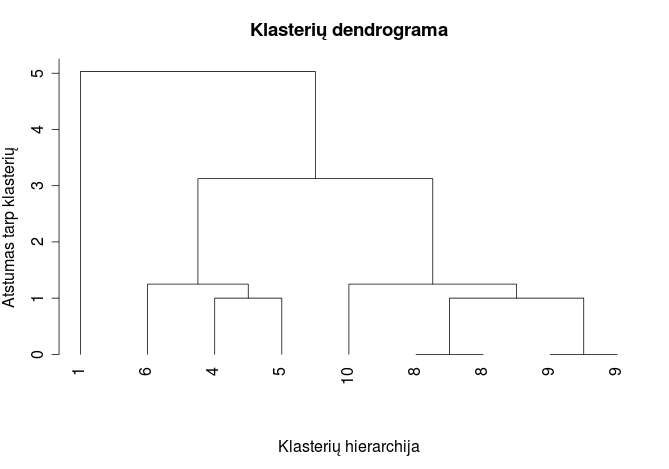
\includegraphics[width=0.6\textwidth]{images/hierarchical_clustering.png}
 \caption{Hierarchinio klasterizavimo rezultatų grafinis pavyzdys.}
 \label{fig:hierarchical_clustering}
\end{figure}
% Šio skyrelio reikia, nes Consensus Group Stable matų atrinkimo metodas naudoja hierarchinio klasterizavimo algoritmą

Hierarchinis klasterizavimas (angl. \textit{hierarchical clustering}) yra klasterizavimo algoritmas, kuris arba visą duomenų aibę panariui skaido į vis mažesnius klasterius (angl. \textit{divisive clustering}), arba pradeda nuo klasterių sudarytų tik iš vieno objekto ir kiekvienoje iteracijoje sujungia panašiausius klasterius (angl. \textit{agglomerative clustering}) \cite{DBLP:books/mk/HanK2000}.  Hierarchinio klasterizavimo rezultatas -- klasterių medis, dendrograma, rodanti, kaip klasteriai yra hierarchiškai susiję. Pasirinktame lygyje nupjovus dendrogramą gaunama klasterizavimo struktūra \cite{martisiute08}. Klasterių dendrogramos pavyzdys yra pateiktas \ref{fig:hierarchical_clustering} pav. Hierarchinis klasterizavimas yra informatyvesnis nei paprastas -- plokščias -- klasterizavimas. Tačiau šių algoritmų sudėtingumas didesnis nei, pvz. tankiu grįstų algoritmų \cite{DBLP:books/mk/HanK2000}.

\subsection{Mokymosi su mokytoju ir mokymosi be mokytojo palyginimas}

 Mokymosi su ir be mokytojo procesai panašūs savo esme -- siekia išgauti žinias apie turimus duomenis, tačiau jų panaudojimas skiriasi iš esmės:
\begin{itemize}
  \item Mokymosi duomenys -- mokymosi su mokytoju proceso įeities duomenyse yra išreikštinai pasakyta, kokio rezultato mes laukiame, o mokymosi be mokytojo įeities duomenyse tokios papildomos informacijos nėra.
  \item  Naudojimo tikslai -- mokymasis su mokytoju siekia iš pavyzdžių išmokti vertinti naujus duomenis, o mokymasis be mokytojo siekia atrasti vidinę duomenų struktūrą.
\end{itemize}

%% JG: aš nesutinku, kad abiem procesais siekiama tųÂ pačių tikslų. Vienu atveju 
% siekiama išmokti iš pavyzdžių. Kitu atveju siekiama atrasti nežinomas
% struktūras turimuose duomenyse. Procesai yra panašūs savo esme, bet jų 
% panaudojimas skiriasi iš esmės.

%% JG: iš vikipedijos: In machine learning, unsupervised learning refers to the 
% problem of trying to find hidden structure in unlabeled data. Since the
% examples given to the learner are unlabeled, there is no error or reward
% signal to evaluate a potential solution. This distinguishes unsupervised 
% learning from supervised learning and reinforcement learning.

%% JG: visą šitą skyrių reikia pateikti koncentruotai. Esminiai teiginiai ir grafiniai pavyzdžiai. 

%% DJ: Turiu pripažint, kad šitam pavyzdyje prigrybavau stipriai. Nurašinėjau
% pavyzdį kur prastai paaiškino skirtumą, bet užtat man pavyzdys patiko. Dabar
% labiau į temą surašyta.

\subsection{Kombinuotasis mokymasis}

Kombinuotasis mokymasis (angl. \textit{ensemble learning}) - tai toks mašininis mokymasis, kai problemos sprendimui yra kombinuojami keli mašininio mokymos metodai. Pristatant kombinuotąjį mokymąsi bus kalbama apie klasifikavimą, tačiau principai yra pritaikomi ir kitiems mašininio mokymosi metodams, pvz. matų atrinkio uždaviniams. 

Kombinuotasis mokymasis pirmiausia yra naudojamas tam, kad pagerintų kuriamo klasifikatoriaus tikslumą arba sumažintų prasto klasifikatoriaus sukūrimo tikimybę. Prielaidos šiam teiginiui yra:
\begin{enumerate}
 \item 
\end{enumerate}



\subsection{Atraminių vektorių klasifikatoriai}

Atraminių vektorių klasifikatoriai (angl. \textit{support vector machines}, SVM) - tai mašininio mokymosi algoritmas, kuris gali būti taikomas tiek klasifikavimui, tiek regresinei analizei. Šis algoritmas priskiriamas prie mokymosi su mokytoju algoritmų \cite{vapnik2000nature}.

Atraminiai vektoriai (angl. \textit{support vectors}) yra mėginiai esantys arčiausiai atskiriančiosios hiperplokštumos (angl. \textit{decision boundary}). Atraminių vektorių klasifikatorių algoritmo tikslas yra mėginių erdvėje orientuoti atskiriančiąją hiperplokštumą tokiu būdu, galimai pašalinant triukšmą bei išimtis (angl. \textit{outlier}), kad atstumas tarp jos ir artimiausių objektų iš abiejų klasių būtų didžiausias \cite{cortes1995support}. Atskiriančiosios tiesės pavyzdys pavaizduotas \ref{fig:support_vector_machines} pav.

Tarkime, kad turime $L$ mokymosi objektų, kurių kiekvienas objektas $x_i$ turi $D$ matų ir priklauso vienai iš dviejų klasių $y_i=-1$ arba $y_i=+1$. Taigi turime mokymosi duomenis, kurių pavidalas yra:
\begin{equation}
 \{x_i, y_i\}, kur\; i=1..L, y_i \in \{-1,1\}, x \in \Re^D
\end{equation}
Tarkime, kad duomenys yra tiesiškai atskiriami. Tai reiškia, kad galima nupiešti tiesę grafe $x_1$ ir $x_2$, kuri atskiria dvi klases, kai $D=2$ ir hiperplokštumą grafuose $x_1, x_2,...x_D$, kai $D > 2$. Hiperplokštuma apibrėžta $w\cdot x_i + b = 0$, kur $w$ -- hiperplokštumos normalės vektorius, $\frac{b}{||w||}$ -- statmens einančio nuo hiperplokštumos iki koordinačių pradžios taško ilgis.

 Taigi, atraminių vektorių klasifikatorių sukūrimas yra parametrų $w$ ir $b$ tenkinančių minėtas sąlygas radimas. Tai galima užrašyti tokia nelygybe:
\begin{equation}
 \label{svm_separable}
 y_i(x_i \cdot w + b) - 1 > 0
\end{equation}
Jei abiejų klasių objektai nėra tiesiškai atskiriami, reikia ,,atpalaiduoti'' (\ref{svm_separable}) salygą įvedant parametrą $\xi_i$:
\begin{equation}
 \label{svm_non_separable}
 y_i(x_i \cdot w + b) - 1 + \xi_i > 0, kur\; \xi_i \geq 0, \;  \forall_i,
\end{equation}
kur $\xi_i$ yra baudos dydis už neteisingai klasei priskirtą mėginį.
\begin{figure}
 \centering
 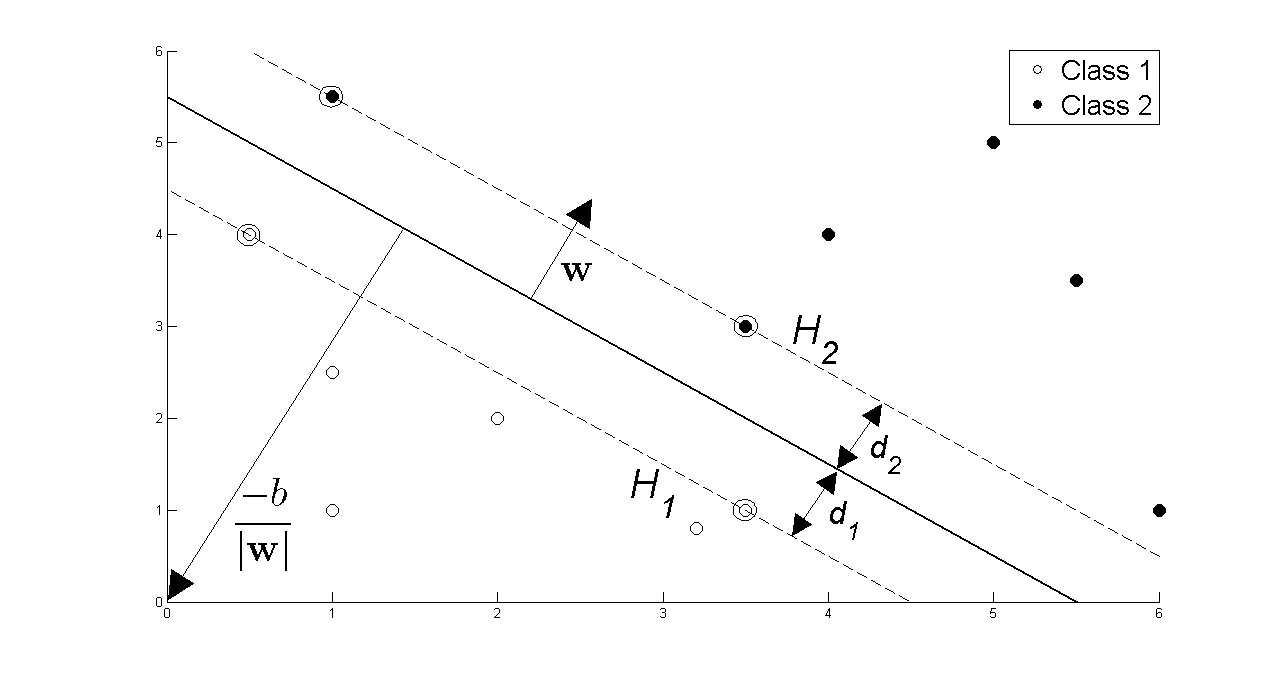
\includegraphics[width=.7\textwidth]{images/support_vector_machines.jpg}
 \caption{Hiperplokštuma nubrėžta per dvi tiesiškai atskiriamas klases.}
 \label{fig:support_vector_machines}
\end{figure}

Atraminių vektorių klasifikatorių algoritmo naudojimas dirbant su biomedicininiais duomenimis populiarus, nes jis demonstruoja gerus rezultatus, kai turima maža daugiamačių mokymosi duomenų aibė. 

%% JG: cituoti turi originalų darbą:
%% JG: C. Cortes and V. Vapnik, Support-Vector Networks, Machine Learning, 20(3):273-297, September 1995
%% JG: Vladimir N. Vapnik. The Nature of Statistical Learning Theory. Springer, New York, 1995

%SVM is a type of machine learning algorithm derived from statistical learning
%[theory](http://download.oracle.com/docs/cd/B14117_01/text.101/b10729/classify.htm).

%% JG: nepamiršksio daugiamatiškumo erdvę, o ten juos galima atskirti tiesiškai.

\subsection{\textit{Random Forest} klasifikatorius}

\textit{Random Forrest} klasifikatorius yra įrankis, kuris sukuria keletą klasifikavimo medžių (angl. \textit{decision tree}), kurie visi nepriklausomai klasifikuoja mėginius, ir daugumos balsavimo (angl. \textit{majority voting}) būdų yra skelbiamas galutinis klasifikavimo rezultatas \cite{breiman1984classification}. Toks daugelio klasifikatorių panaudojimas yra vadinamas kombinuotoju mokymusi (angl. \textit{ensemble learning}). 

Kiekvienas klasifikavimo medis yra konstruojamas pagal procedūrą aprašytą algoritme nr. \ref{random_forest_algorithm}.

\begin{algorithm}
 \caption{\textit{Random Forest} klasifikavimo medžių konstravimas}
 \label{random_forest_algorithm}
 \begin{enumerate}
  \item Turimas $N$ mėginių, kurie turi $M$ matų;
  \item Pasirenkamas $m$ matų, kurie bus naudojami klasifikavimo medžių kūrimui; $m << M$;
  \item Sudaroma treniravimosi mėginių aibė $n$ kartų pasirenkant mėginius su pasikartojimais iš visų $N$ mėginių. Visi nepasirinkti mėginiai paliekami klasifikatoriaus testavimui; 
  \item Kiekvienam medžio mazgui atsitiktinai pasirinkama $m$ matų, kuries sudarys sąlygą tam mazgui. Randamas geriausia atskyrimo sąlyga treniravimos duomenims pagal tuos $m$ matų;
  \item Pilnai užauginti medžiai nėra genėjami (angl. \textit{pruning}).
 \end{enumerate}
\end{algorithm}

\textit{Random forest} algoritmo tikslumas priklauso nuo: koreliacijos tarp sukurtų klasifikavimo medžių (didesnė koreliacija lemia mažesnį klasifikavimo tikslumą.); atskiro klasifikavimo medžio skiriamoji galia (kuo didesnė atskiro klasisifikavimo medžio skiriamoji galia, tuo geresnis klasifikavimo tikslumas).

\textit{Randon forest} klasifikatoriai yra tikslūs, greiti, bei sugeba išvengti persimokymo (angl. \textit{overfitting}). Šios trys klasifikavimo algoritmo savybės yra labai svarbios dirbant su biomedicininiais duomenimis. 

\newpage

\section{PAGRINDINIAI MATŲ ATRINKIMO METODAI}
\label{pagrindiniai_matu_atrinkimo_motodai}

Dėl ,,daugiamatiškumo prakeiksmo`` (angl. \textit{the curse of dimentionality}) -- didėjant matų kiekiui mėginiai pasidaro panašūs, todėl bandymas juos klasifikuoti tolygus spėliojimui \cite{bellman1966adaptive}. Biomedicininių duomenų kontekste galima daryti prielaidą, kad ne visi matai yra susiję su tiriama problema, pvz. gaubtinės žarnos vėžiu, dėl to, kad duomenys yra daugiamačiai. Paprastai nagrinėjamai problemai svarbus yra mažas, palyginus su visu, matų kiekis. Todėl biomedicininių duomenų daugiamatiškumui sumažinti yra naudojami informatyviausių matų atrinkimo metodai \cite{guyon2003introduction} (angl. \textit{feature selection}). Matų atrinkimas yra svarbi biomedicininių duomenų apdorojimo (angl. \textit{preprocessing}) etapo dalis. Naudojant matų atrinkimo metodus, galima kovoti su daugiamatiškumo prakeiksmu matų skaičių priartinant prie mėginių skaičiaus. Todėl svarbu yra pasirinkti geriausiai tinkančią matų atrinkimo strategiją. Kadangi ir pačių matų atrinkimo metodų veikimas priklauso nuo 
konkrečių duomenų, tai metodo pasirinkimas yra sudėtinga užduotis.

Pagal tai, kaip matų atrinkimo metodai yra susiję su klasifikatoriumi, matų atrinkimo metodus galima skirstyti į tris kategorijas \cite{saeys2008robust}:
\begin{enumerate}
 \item Filtruojantys metodai (angl. \textit{filter methods}), pvz. \textit{Fisher} įvertis. Jie dirba tiesiogiai su duomenimis, o jų darbo rezultatas gali būti matų įvertinimas svoriais, matų reitingavimas ar tiesiog geriausių matų poaibis, kuriuo remiantis vėliau apmokomas klasifikatorius. Tokių metodų pagrindinis privalumas yra tai, kad jie yra greiti, tinka paskirstytų skaičiavimų aplinkoms ir nepriklausomi nuo klasifikavimo  metodo, tačiau remiantis atrinktaisiais matais nebūtinai bus sukurtas geriausias klasifikatorius.
 \item Prisitaikantieji metodai (angl. \textit{wrapper methods}). Pirma, apmokomas klasifikatorius su visais matais, antra, parenkamas matų poaibis ir apmokomas klasifikatorius. Po daugkartinio matų aibių įvertinimo pagal klasifikavimo rezultatus yra nusprendžiama, kuris matų poaibis yra labiausiai tinkamas klasifikavimui. Įterptinių metodų atveju matų atrinkimo procesas yra neatsiejamas nuo klasifikavimo proceso -- matai yra atrenkami pagal klasifikatoriaus darbo rezultatus. Prisitaikantieji metodai dažnai duoda geresnius rezultatus negu filtravimo metodai, bet yra reiklūs resursams.
 \item Įterptiniai metodai (angl. \textit{embedded methods}), pvz. AW-SVM\cite{vapnik2000nature}. Jie matų atrinkimui naudoja vidinius klasifikatoriaus duomenis (pvz. matų svoriai gauti pagal SVM). Šie metodai dažnai siūlo gerą santykį tarp klasifikavimo tikslumo ir skaičiavimų sudėtingumo.
\end{enumerate}

Šiame skyriuje nagrinėsiu pagrindinius matų atsirinkimo metodus:
\begin{enumerate}
 \item \textit{Fisher} įvertis (angl. \textit{Fisher ratio})\cite{Pavlidis:2001:GFC:369133.369228};
 \item \textit{Relief} metodas\cite{DBLP:journals/ml/Robnik-SikonjaK03};
 \item Asimetrinis priklausomybės koeficientas (angl. \textit{Asymmetric Dependency Coefficient, ADC}) \cite{Shannon:2001:MTC:584091.584093};
 \item Absoliučių svorių SVM (angl. \textit{Absolute Weight SVM}, AW-SVM) \cite{vapnik2000nature};
 \item Rekursyvus matų eliminavimas pagal SVM (SVM-RFE) (angl. \textit{Recursive Feature Elimination by SVM}) \cite{Guyon:2002:GSC:599613.599671}.
\end{enumerate}

\subsection{\textit{Fisher} įvertis}

\textit{Fisher} įvertis vertina individualius matus pagal matų klasių atskiriamąją galią. Mato įvertis yra sudarytas iš tarpklasinio skirtumo santykio su vidiniu klasės pasiskirstymu:
\begin{equation}
 FR(j) = \frac{(\mu_{j1} - \mu_{j2})^2}{\sigma_{j1}^2 + \sigma_{j2}^2},
\end{equation}
kur, 
$j$ -- yra mato indeksas, 
$\mu_{jc}$ -- mato $j$ reikšmių vidurkis klasėje $c$, 
$\sigma_{jc}^2$ -- mato $j$ reikšmių standartinis nuokrypis klasėje $c$, kur $c={1,2}$. Kuo didesnis yra \textit{Fisher} įvertis, tuo geriau ts matas atskiria klases. Nors ir paprastas, šis metodas neįvertina matų tarpusavio sąveikų.

\subsection{\textit{Relief} metodas}

\textit{Relief} metodas iteratyviai skaičiuoja matų ,,susietumą``. Pradžioje ,,susietumas`` visiems matams yra lygus nuliui. Kiekvienoje
iteracijoje atsitiktinai pasirenkamas mėginys iš mėginių aibės, surandami artimiausi kaimynai iš tos pačios ir kitos grupių, ir atnaujinamos visų 
matų ,,susietumo`` reikšmės. Dėl atsitiktinumo faktoriaus klasifikavimo ir  matų atrinkimo stabilumo rezultatai naudojant šį metodą varijuoja. Mato įvertis yra vidurkis visų objektų atstumų skirtumų iki artimiausių kaimynų iš kitos ir tos pačios klasių:
\begin{equation}
 W(j)=W(j) - \frac{diff(j, x, x_H)}{n} + \frac{diff(i, x, x_M)}{n},
\end{equation}
kur 
$W(j)$ -- $j$-ojo mato ,,susietumo`` įvertis, 
$n$ -- mėginių aibės dydis, 
$x$ -- atsitiktinai pasirinktas mėginys, 
$x_H$ - artimiausias $x$ kaimynas iš tos pačios grupės (angl. \textit{nearest-Hit}), 
$x_M$ -- artimiausias $x$ kaimynas iš kitos grupės (angl. \textit{nearest-Miss}),
$diff(j, x, x')$ -- $j$-ojo mato reikšmių skirtumas tarp atsitiktinai pasirinkto objekto $x$ ir atitinkamo jo kaimyno, kur skirtumą į intervalą $[0, 1]$ normalizuojanti funkcija yra:
\begin{equation}
 diff(j, x, x')=\frac{|x_j- x_j'|}{x_{j_{max}} - x_{i_{min}}},
\end{equation}
kur $x_{j_{max}}$ ir $x_{j_{min}}$ yra maksimali ir minimali $j$-ojo matų reikšmės. ,,Susietumo`` reikšmių atnaujinimas yra vykdomas $n$ kartų ir kuo didesnė galutinė reikšmė, tuo svarbesnis matas. Šis algoritmas atsižvelgia į matų tarpusavio priklausomybes, nes mėginio artimiausias kaimynas yra ieškomas pagal visus mėginį apibūdinančius matus. Aprašyta algoritmo versija yra skirta dviejų klasių atvejui, tačiau yra ir multiklasinis algoritmo variantas \cite{DBLP:journals/ml/Robnik-SikonjaK03}.

\subsection{Asimetrinis priklausomybės koeficientas}

Asimetrinis priklausomybės koeficientas (angl. \textit{asymetric dependency coefficient}, ADC) yra matų reitingavimo motodas, kuris matuoja mėginio grupės tikimybinę priklausomybę $j$-ajam matui, naudodamas informacijos prieaugį (angl. \textit{information gain}) \cite{kent1983information}:
\begin{equation}
 ADC(Y, j) = \frac{MI(Y, X_j)}{H(Y)},
\end{equation}
kur $H(Y)$ -- klasės $Y$ entropija (angl. \textit{entropy}), o $MI(Y, X_j)$ -- yra tarpusavio informacija \cite{Shannon:2001:MTC:584091.584093} (angl. \textit{mutual information}) tarp mėginio grupės $Y$ ir $j$-ojo mato.
\begin{equation}
 H(Y)=-\sum_y{p(Y=y)log{p(Y=y)}}, 
\end{equation}
\begin{equation}
 H(X_j)=-\sum_x{p(X_j=x) log{p(X_j=x)}},
\end{equation}
\begin{equation}
 MI(Y, X_j) = H(Y) + H(X_j) - H(Y, X_j),
\end{equation}
\begin{equation}
 H(Y, X_j) = -\sum_{y,x_j}{p(y, x_j)log{p(y, x_j)}},
\end{equation}
Kuo didesni ADC įverčiai, tuo matas yra svarbesnis, nes turi daugiau informacijos apie mėginio priklausomybę grupei.

\subsection{Absoliučių svorių SVM}

Atraminių vektorių klasifikatorius (SVM) yra vienas populiariausių klasifikavimo algortimų, nes jis gerai susidoroja su daugiamačiais duomenimis \cite{guyon2002gene}. Yra keletas bazinių SVM variantų \cite{vapnik2000nature}, bet šiame darbe naudosime tiesinį SVM, nes jis demonstruoja gerus rezultatus analizuojant genų ekspresijos duomenimis. Tiesinis SVM yra hiperplokštuma apibrėžta kaip:
\begin{equation}
 \sum_{j=1}^{p}{w_jx_j + b_0 = 0},
\end{equation}
kur $p$ -- matų kiekis, $w_j$ -- j-ojo mato svoris, $x_j$ -- j-ojo mato kintamasis, $b_0$ -- konstanta. Mato absoliutus svoris $w_j$ gali būti panaudotas
matų reitingavimui. Svorį reikia imti absoliutaus dydžio, nes neigiamas svoris implikuoja priklausomybę vienai grupei, o teigiamas kitai grupei. Pastebėtina, kad svorių nustatymas yra atliekamas tik vieną kartą (SVM-RFE matų atrinkimo metodas svorius matams nustato daug kartų).

\subsection{Rekursyvus matų eliminavimas pagal SVM}

Rekursyvus matų eliminavimas pagal SVM (angl. \textit{Support Vector Machines -- Recursive Feature Elimination}, SVM-RFE) yra vienas populiariausių matų atrinkimo algoritmų \cite{guyon2002gene}. Todėl, jis yra naudojamas kaip atskaitos taškas (angl. \textit{benchmark}) vertinant kitus matų atrankos metodus. Iš esmės šis metodas yra daugkartinis absoliučių svorių SVM metodo taikymas nuolat išmetinėjant matus su mažiausiais svoriais. Rekursyvus matų eliminavimas mums padeda surasti tinkamą matų poaibį, kas ne visada pavyksta su matų reitingavimo metodais. Bendroji rekursyvaus matų eliminavimo procedūra:
\begin{algorithm}
\caption{Rekursyvus matų eliminavimas}
\label{RFE}
 \begin{enumerate}
 \item Turime pilną matų rinkinį $F_0$, nustatome $i=0$;
 \item Įvertiname kiekvieno mato kokybę matų aibėje $F_i$;
 \item Išmetame mažiausiai kokybišką matą iš $F_I$ tam, kad gautume matų rinkinį $F_{i+1}$;
 \item Nustatome $i=i+1$ ir grįžtame į antrąjį žingsnį kol nėra patenkinta algoritmo pabaigos sąlyga.
\end{enumerate}
\end{algorithm}
Jei trečiajame algoritmo žingsnyje iš matų aibės yra pašalinamas tik viena matas, tai gauname matų reitingavimą, o jei pašalinamas fiksuotas skaičius ar dalis (pvz. 50\%) matų, tai matų reitingavimo negauname. Pastebėtina, kad rekursyvus matų eliminavimas labai padidina algoritmo sudėtingumą. Algoritmo pabaigos sąlyga gali būti koks nors konkretus matų skaičius arba tiesiog matų aibę mažiname tol, kol matų visai nebeliks.

\section{STABILIŲ MATŲ ATRINKIMO METODAI}
\label{stabiliu_matu_atrinkimo_metodai}

Naudodami matų atrinkimo metodus, biomedicininius duomenis tiriantys mokslininkai susiduria su atrinktųjų matų aibės stabilumo problema - atrenkant matus pagal kitą mėginių poaibį, gaunamas kitas informatyviausių matų poaibis. Matų atrinkimo nestabilumas yra sąlygotas šių veiksnių:
\begin{enumerate}
 \item Duomenys yra triukšmingi ir kai kurie matai gali būti palaikyti informatyviais dėl atsitiktinių priežasčių;
 \item Daugiamačiuose duomenyse tikėtina, kad dalis matų koreliuoja, todėl, kuris iš koreliuojančių matų bus pasirinktas, priklauso nuo to, kuriuos mėginius pasirinksime klasifikatoriaus apmokymui;
 \item Kiekvienas maatų atrinkimo algoritmas daro skirtingas prielaidas apie tai, kurie matai yra informatyvūs.
\end{enumerate}
Galime teigti, kad skirtingi metodai tiems patiems duomenims gali atrinkti skirtingus matus. Taip pat, suskaidžius turimus duomenis į atskiras persidengiančias aibes ir atrinkus tą patį kiekį matų tuo pačiu metodu, gaunamos skirtingos matų aibės. Be to, kuo triukšmingesni duomenys, kuo mažiau turima mėginių ir kuo daugiau yra matų, tuo ryškesnė yra ši problema \cite{loscalzo2009consensus}. 

Vienas iš būdų didinti matų atrinkimo stabilumą yra naudoti multikriterinius matų atrinkimo metodus. Jų esmė yra panaudoti kelis matų atrinkimo metodus suliejant jų rezultatus į vieną bendrą rezultatą. Yra skiriamos trys priežastys, kodėl keletas agreguotų silpnų ir nestabilių matų atrinkimo metodų gali duoti stabilesnius matų atrinkimo rezultatus \cite{dietterich2000ensemble}:
\begin{enumerate}
 \item Keletas skirtingų, bet vienodai optimalių hipotezių gali būti teisingos, ir kriterijų agregavimas sumažiną tikimybę, kad bus pasirinkta neteisinga  hipotezė;
 \item Atskiri matų atrinkimo metodai gali dirbti skirtinguose lokaliuose optimumuose, tuo tarpu agregavimas gali geriau reprezentuoti tikrąją  duomenis generuojančią funkciją;
 \item Tikroji duomenų funkcija negali būti reprezentuojama jokia hipoteze paskiro algoritmo hipotezių erdvėje ir agreguojant pavienių metodų rezultatus galima praplėsti hipotezių erdvę.
\end{enumerate}
Apibendrinant galima sakyti, kad suliejant keletą skirtingų matų atrinkimo metodų rezultatų suliejamos gerosios pavienių matų atrinkimo metodų savybės, taip bandant kompensuoti tų algoritmų silpnybes.

Šiame skyriuje aptarsiu matų atrinkimo stabilumą didinančius metodus:
\begin{enumerate}
 \item Svoriais grįstas multikriterinis suliejimas;
 \item Reitingais grįstas multikriterinis suliejimas;
 \item Svoriais ir reitingais grįstas multikriterinis suliejimas;
 \item Multikriterinis rekursyvus matų eliminavimas;
 \item Konsensuso grupėmis grįstas stabilių matų atrinkimo metodas.
\end{enumerate}

\subsection{Svoriais grįstas multikriterinis suliejimas}

Svoriais grįsto multikriterinio matų atrinkimo suliejimo pagal svorius algoritmo pirmajame žingsnyje kiekvienas bazinis metodas priskiria duomenų rinkinio matams svorius, tada tie svoriai yra kombinuojami į vieną sutarties (angl. \textit{consensus}) svorių vektorių, kurio pagrindu yra gaunami matų reitingai. Algoritmas yra pavaizduotas ~\ref{fig:figure4} pav.
\begin{figure}
 \centering
 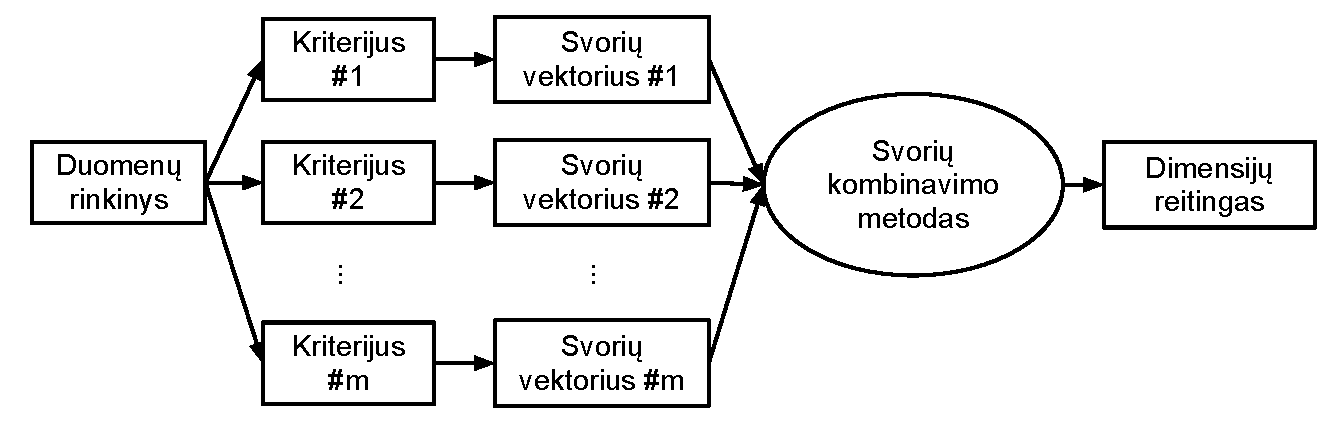
\includegraphics[width=1\textwidth]{images/score_based_fusion.pdf}
 \caption{Svoriais grįstas multikriterinis suliejimas.}
 \label{fig:figure4}
\end{figure}

\begin{figure}[ht]
\begin{minipage}[b]{0.45\linewidth}
\centering
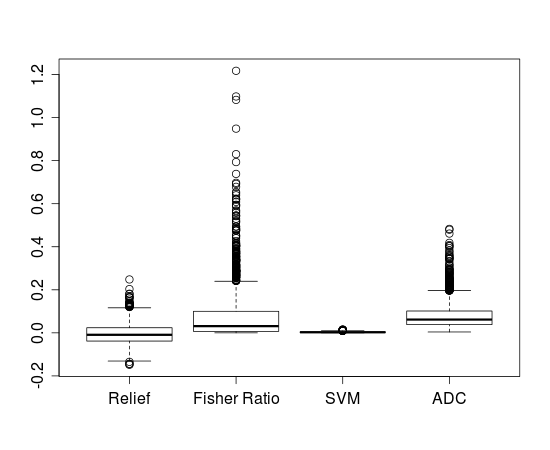
\includegraphics[width=1\textwidth]{images/boxplot_colon_all.png}
\caption{Pavienių matų atrinkimo metodų nenormalizuotas svorių pasiskirstymas.}
\label{fig:figure1}
\end{minipage}
\hspace{0.2cm}
\begin{minipage}[b]{0.45\linewidth}
\centering
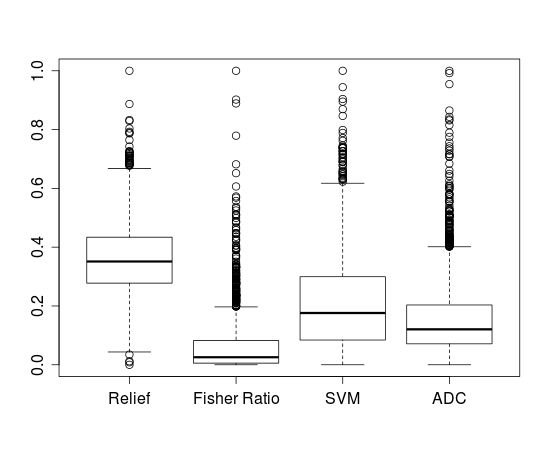
\includegraphics[width=1\textwidth]{images/boxplot_colon_all_normalized.png}
\caption{Pavienių matų atrinkimo metodų normalizuotas svorių pasiskirstymas.}
\label{fig:figure2}
\end{minipage}
\end{figure}

Suliejant svorius svarbu yra užtikrinti, kad svoriai, gauti naudojant skirtingus bazinius kriterijus, būtų palyginami. Todėl svorių normalizavimas turi būti atliekamas prieš svorių kombinavimą. Kitu atveju matų įvertinimai bus nepalyginami. Paveikslėlyje ~\ref{fig:figure1} pav. nenormalizuotų pavienių matų vertinimo metodų skiriasi netgi suteiktų svorių intervalai. Paveikslėlyje ~\ref{fig:figure2} pav. matome, kad net ir normalizavus svorius skiriasi svorių kvartiliai -- į tai reikia atkreipti dėmesį interpretuojant galutinius matų vertinimo rezultatus. Šiame darbe svoriai yra normalizuoti intervale $[0, 1]$ pagal formulę:
\begin{equation}
 u_i'=\frac{u_i - u_{i_{min}}}{u_{i_{max}} - u_{i_{min}}}, 
\end{equation}
kur $u_i$ - matų svorių vektorius pagal $i$ kriterijų, 
$u_{i_{min}}$ - minimali $u_i$ svorių vektoriaus reikšmė,
$u_{i_{max}}$ - maksimali $u_i$ svorių vektoriaus reikšmė,
$u_i'$ - normalizuotų svorių vektorius.

Sutarties svorių vektorius $u$ yra vidurkis normalizuotų svorių vektorių:
\begin{equation}
 u = \frac{1}{m}\sum_{i=1}^m u_i',
\end{equation}
kur $m$ yra bazinių kriterijų skaičius. Reikia paminėti, kad didesnė svorio reikšmė reiškia, kad matas yra reikšmingesnis klasifikavimui.

\subsection{Reitingais grįstas multikriterinis suliejimas}

Reitingais grįsto multikriterinio suliejimo pagal reitingus metodas gauna mėginių aibę aprašančių matų reitingą, pagal keletą bazinių matų reitingavimo kriterijų. Algoritmo pirmajame žingsnyje keletas matų atrinkimo kriterijų grąžina matų reitingus, paskui tie reitingai yra kombinuojami į vieną bendra matų reitingą. Algoritmas yra
pavaizduotas ~\ref{fig:figure5} pav.
\begin{figure}
 \centering
 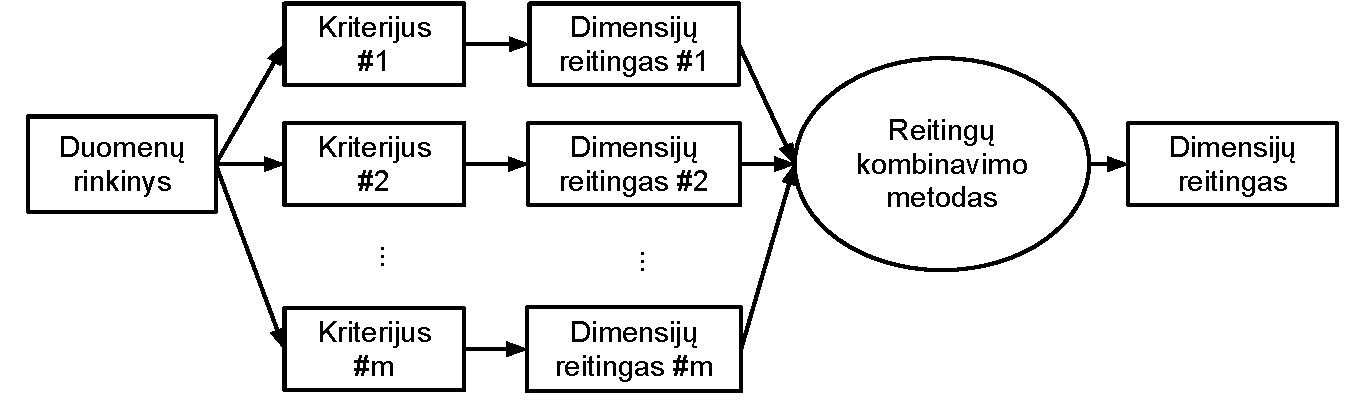
\includegraphics[width=1\textwidth]{images/ranking_based_fusion.pdf}
 \caption{Reitingais grįstas multikriterinis suliejimas.}
 \label{fig:figure5}
\end{figure}
Suliejimo pagal reitingus metodas nereikalauja matų atrinkimo metodų rezultatų normalizavimo, todėl galima matams priskirtus reitingus kombinuoti iškart. Skirtingai nei suliejimo pagal svorius algoritme, baziniai matų atrinkimo kriterijai turi gražinti matų reitingus, o ne svorius.

Matų reitingų kombinavimui yra keletas metodų\cite{dwork2001rank}, tačiau paprastumo dėlei šiame darbe naudosiu Borda balsavimą\footnote{Dar žinomas kaip ,,Pažymių metodas``. Jis buvo pasiūlytas prancūzų matematiko ir fiziko Jean-Charles de Borda 1770 metais.} (angl.\textit{ Borda count}). Tarkime, kad turime $m$ basuotojų ir $p$ kandidatų aibę. Tada Borda balsavimo metodas kiekvienam $i$-ajam balsuotojui sukuria balsų vektorių $v_i$ tokiu būdu: geriausiai įvertintam kandidatui suteikiama $p$ taškų, antrajam kandidatui $p-1$, ir t.t. Galutiniai taškai yra gaunami sudedant visų balsuotojų taškus
\begin{equation}
 v = \sum_{i=1}^m v_i,
\end{equation}
kur $v$ yra suminių taškų vektorius, o iš jo galime gauti ir galutinius matų reitingus.

\subsection{Svoriais ir reitingais grįstas multikriterinis suliejimas}

Svoriais ir reitingais grįsto multikriterinio suliejimo metodas nuo reitingais grįsto multikriterinio suliejimo metodo skiriasi tuo, kad kaip dar vienas matų reitingas yra panaudojamas svoriais grįsto multikriterinio matų atrinkimo metu gautas reitingas. Multikriterinio matų įverčių ir pagal svorius, ir pagal reitingus metodas vyksta trimis žingsniais:
\begin{enumerate}
  \item Gauname matų reitingus pagal $m$ pavienių matų atrinkimo motodų;
  \item Suliejame matų įverčius pagal svorius, taip gauname vieną matų reitingą;
  \item Reitinguojame matus pagal visus turimus $m+1$ pavienius reitingus.
\end{enumerate} 
Algoritmas yra pavaizduotas ~\ref{fig:figure3} pav.
\begin{figure}
 \centering
 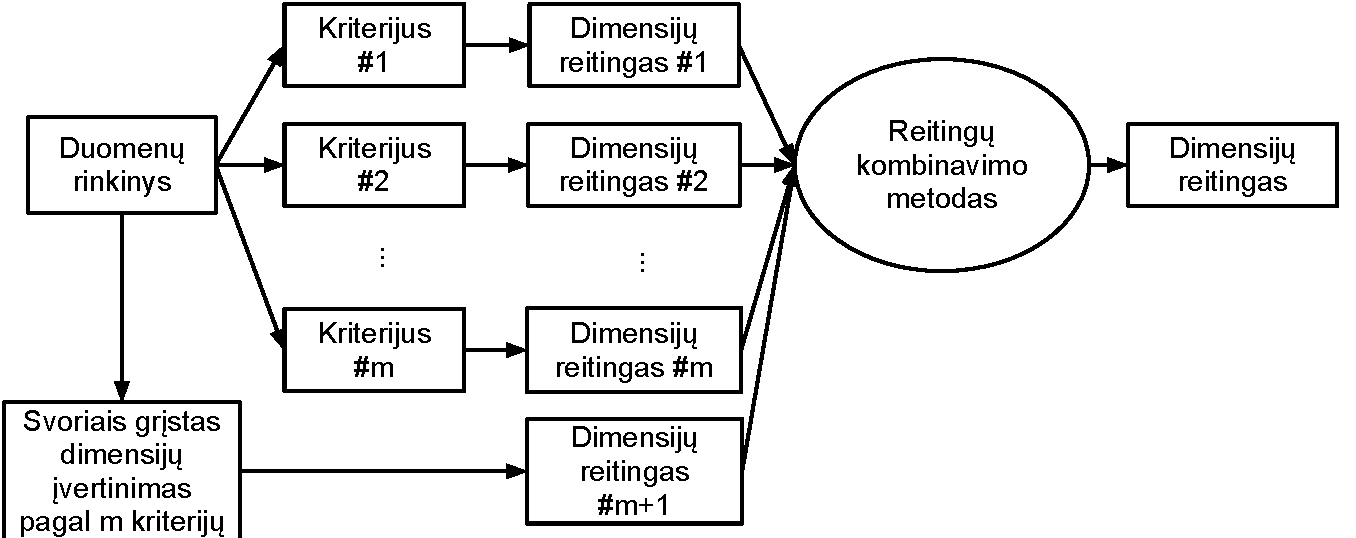
\includegraphics[width=1\textwidth]{images/score_and_ranking_based_fusion.pdf}
 \caption{Svoriais ir reitingais grįstas multikriterinis suliejimas.}
 \label{fig:figure3}
\end{figure}

Suliejami keletą mažai koreliuojančių matų reitingavimo metodų rezultatų, yra siekiama didesnio matų atrinkimo stabilumo, kai varijuoja treniravimosi duomenų poaibis (angl. \textit{subsampling}) \cite{yang2011robust}.

\subsection{Multikriterinis rekursyvus matų eliminavimas}

Jei matų atrinkimo tikslas yra pagerinti klasifikavimo rezultatus, tai taikymas multikriterinių matų atrinkimo metodų nebūtinai duos pageidaujamą rezultatą, nes yra pastebėta, kad vien matų reitingavimas nebūtinai suranda geriausią matų poaibį. Tam, kad būtų surastas geriausias matų poaibis reikia kombinuoti multikriterinį matų reitingavimą su matų paieškos strategija. Rekursyvus matų eliminavimas yra dažnai naudojama matų paieškos strategija matų atrinkimui. Todėl yra kombinuojamas multikriterinis matų reitingavimas ir rekursyvus matų eliminavimas.

Multikriterinis rekursyvus matų eliminavimas susideda iš dviejų dalių \cite{yang2011robust}: keletos matų atrinkimo kriterijų suliejimo pagal svorius ir pagal reitingus, ir rekursyvaus matų eliminavimo aprašyto algoritme nr. \ref{RFE}. Algoritmas pavaizduotas ~\ref{fig:figure6} pav.
\begin{figure}
 \centering
 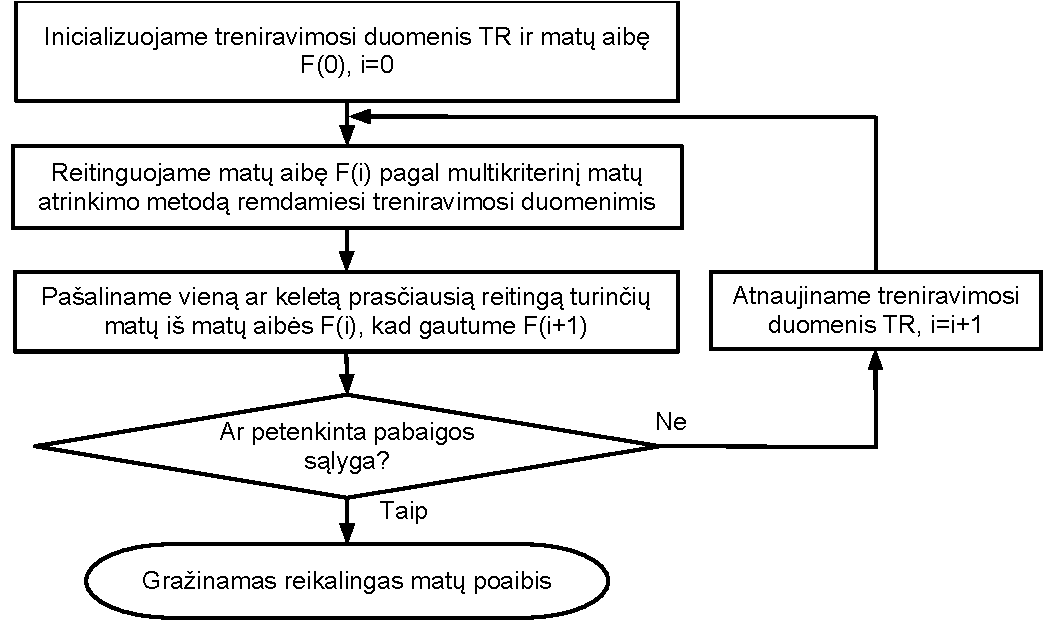
\includegraphics[width=0.7\textwidth]{images/mcf-rfe_procedure.pdf}
 \caption{Multikriterinio rekursyvaus matų eliminavimo algoritmas.}
 \label{fig:figure6}
\end{figure}

Standartinis rekursyvus matų eliminavimas, kai vienos iteracijos metu yra eliminuojamas vienas matas, gali labai padidinti algoritmo sudėtingumą. Todėl genų ekspresijos duomenims prasmingiau yra eliminuoti keletą matų vienu metu.

Nors SVM-RFE matų atrinkimo algoritmas ir yra labai populiarus, tačiau yra žinoma, kad jam trūksta stabilumo \cite{guyon2002gene}. Todėl kombinuodami didesnį stabilumą turintį multikriterinį matų atrinkimą su rekursyvaus matų eliminavimo paieškos strategija, gauname stabilesnį matų atrinkimo algoritmą.

\subsection{Konsensuso grupėmis grįstas stabilių matų atrinkimo metodas}

Konsensuso grupėmis grįstas stabilių matų atrinkimo metodas(angl. \textit{Consensus Group Stable feature selection}, CGS), pirma, identifikuoja panašių matų grupes, antra, pagal surastas grupes transformuoja matų aibę, trečia, transformuotoje matų aibėje atlieka matų atrinkimą \cite{loscalzo2009consensus}. Schematiškai šis algoritmas pavaizduotas ~\ref{fig:figure7} pav. 
\begin{figure}
 \centering
 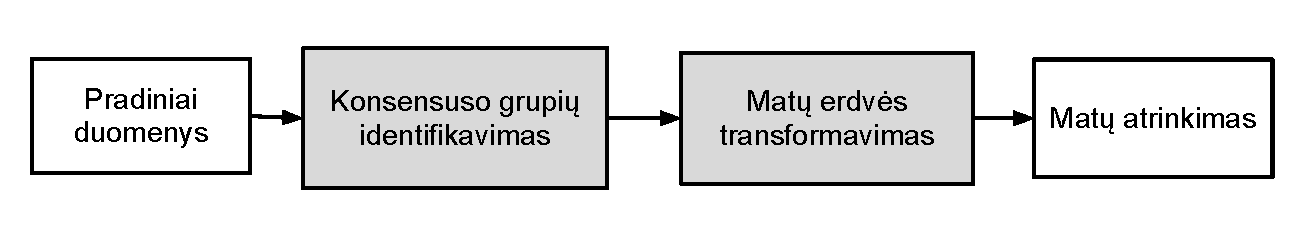
\includegraphics[width=\textwidth]{../bachelor/images/consensus_group_based_feature_selection_framework.pdf}
 \caption{Konsensuso grupėmis grįstas stabilių matų atrinkimas.}
 \label{fig:figure7}
\end{figure}

CGS metodo pagrindinė dalis yra panašių matų identifikavimas. Šio uždavinio sprendimui naudojamas \textit{Dense Group Finder} (DGF) algoritmas. DGF aprašytas algoritme nr. \ref{DGF}. CGS algoritme agal matai pagal DGF algoritmą yra sugrupuojami keletą kartų. Po pakartotinio grupavimo yra ieškoma stabilių grupių -- jei matas buvo sugrupuotas į konkrečią grupę daugiau nei pusėje grupavimų, tai matas ir priklausys tai konsensuso grupei. Matų aibės transformavimas vyksta iš kiekvienos konsensuso grupės išrenkant reprezentatyviausią matą -- konkretų matą esantį arčiausiai konsensuso grupės vidurkio. Išrinktieji reprezentatyviausieji matai ir sudaro transformuotą matų aibę. Transformuotoje matų aibėje vykdomas matų antrinkimas koriuo nors matų atrinkimo metodu $\Phi$, pavyzdžiui, \textit{Relief} matų atrinkimo metodu. 
\begin{algorithm}
\caption{DGF -- \textit{Dense Group Finder}}
\label{DGF}
 \begin{algorithmic}
 \item \textbf{Įeitis:} duomenys $D=\{x_i\}_{i=1}^n$, branduolio plotis $h$
 \item \textbf{Išeitis:} tankios matų grupės $G_1, G_1,..., G_L$
 \For{$i = 1$ \textbf{to} $n$ \do} 
  \State Inicializuojame $j=1, y_{i,j}=x_i$
  \Repeat
    \State Suskaičiuoti tankio centrą $y_{i, j+1}$ pagal (\ref{for_dgf})
  \Until{konverguoja}
  \State Nustatyti tankio centrą $y_{i,c} = y_{i,j+1}$ (Nustatyti piką $p_i$ kaip $y_{i,c}$)
  \State Sulieti piką $p_i$ su artimiausiais pikais, jei atstumai tarp jų $ < h$
 \EndFor
 \item Iš kiekvieno unikalaus piko $p_r$, pridėkime $x_i$ į $G_r$, jei $||p_r - x_i|| < h$
 \end{algorithmic}
\end{algorithm}

\begin{equation}
\label{for_dgf}
  y_{i, j+1}=\frac{\sum_{i=1}^{n} x_i K(\frac{y_j - x_i}{h})}{\sum_{i=1}^{n} K(\frac{y_j - x_i}{h})} j=1,2,...
\end{equation}
kur $K(x)$ -- \textit{kernel} funkcija, $h$ -- \textit{kernel} plotis, $y$ -- tankio centras.

\begin{algorithm}
 \caption{Konsensuso grupėmis grįstas stabilių matų atrinkimas}
 \label{CGS}
 \begin{algorithmic}
   \item \textbf{Įeitis:} mėginių aibė $D$, iteracijų skaičius $t$, matų atrinkimo metodas $\Phi$\
   \item \textbf{Išeitis:} atrinktos konsensuso matų grupės $CG_1, CG_1,..., CG_k$
   \item // Konsensuso grupių identifikavimas
   \For{$i = 1$ \textbf{to} $n$ \do}
    \State Parinkti mėginių  poaibį $D_i$ iš $D$
    \State Gauti panašių matų grupes pagal $DGF(D_i, h)$
   \EndFor
   \For{kiekvienai matų porai $X_i$ ir $X_j \in D$}
    \State Nustatyti $W_{i,j}=$ dažnis, kai $X_i$ ir $X_j$ yra toje pačioje grupėje $/t$
   \EndFor
   \item Sudaryti konsensuso grupes $CG_1, CG_1,..., CG_L$ atliekant hierarchinį klasterizavimą visiems matams pagal $W_{i, j}$
   \item //Matų atrinkimas grįstas konsensuso grupėmis
   \For{$i = 1$ \textbf{to} $l$ \do}
    \State Parinkti reprezentatyvų matą $X_i$ iš $CG_i$
    \State Įvertinti mato informatyvumą $\Phi(X_i)$
   \EndFor
   \item Reitinguoti konsensuso grupes $CG_1, CG_1,..., CG_L$ pagal $\Phi(X_i)$
   \item Pasirinkti $k$ matų, turinčių geriausią reitingą  
 \end{algorithmic}
\end{algorithm}
\newpage

% Čia aprašysiu eksperimentus
\subsection{Naudoti duomenys}

Šiame darbe eksperimentai buvo atliekami su biomedicininiais viešai prieinamais
genų ekspresijos duomenų rinkiniais.
\begin{longtable}{|p{4cm}|p{1.4cm}|p{2.5cm}|p{1.6cm}|p{1cm}|}
\captionsetup{labelsep=period}
\caption{Darbe naudoti duomenų rinkiniai\label{table:datasets}}\\
%This is the header for the first page of the table...
\hline \hline
{\textbf{Pavadinimas}} &
{\textbf{Šaltinis}} &
{\textbf{Objektų skaičius (+/-)}}&
{\textbf{Dimensijų skaičius}}&
{\textbf{ODS}}\\
\hline
\endfirsthead
%This is the header for the remaining page(s) of the table...
\multicolumn{3}{c}{{\tablename} \thetable{} -- Tęsinys} \\[0.5ex]
\hline \hline
{\textbf{Pavadinimas}} &
{\textbf{Šaltinis}} &
{\textbf{Objektų skaičius (+/-)}}&
{\textbf{Dimensijų skaičius}}&
{\textbf{ODS}}\\
\hline
\endhead
%This is the footer for all pages except the last page of the table...
\multicolumn{3}{l}{{Lentelės tęsinys kitame puslapyje\ldots}} \\
\endfoot
%This is the footer for the last page of the table...
\hline \hline
\endlastfoot
\hline 
Gaubtinės žarnos auglys (angl. Colon) 
& 
\cite{alon1999broad} 
& 
62 (40/22) 
& 
2000 
& 
3,1\% \\
\hline
Centrinės nervų sistemos auglys (CNS) 
& 
\cite{pomeroy2002prediction} 
& 
60 (39 AAL / 21 AML) 
& 
7129 
& 
0.84\% \\
\hline
Prostatos auglys 
& 
\cite{singh2002gene} 
& 
102 (52/50) 
& 
6033 
& 
1.7\% \\
\hline
Šizofrenija ir maniakinė depresija
&
\cite{altara}
&
90 (bp\footnote{bp (angl. Bipolar disorder) - maniakine depresija sergantys
pacientai.}:
sz\footnote{sz (angl. Schizophrenia) - šizofrenija sergantys pacientai.}:
cc\footnote{cc (angl. Control Crowd) - kontrolinė grupė.} =30:31:29)
&
22283
&
0.403\% \\
\hline
\end{longtable}
Duomenų rinkinius apibūdinantis dydis ODS, kuris turimiems duomenims tesiekia
nuo  0,403\% iki 3,01\% procento, parodo, kad turime labai retus (angl. sparce) duomenis, o tai labai apsunkina
mokymosi procesą ir gali sukelti persimokymo (angl. overfitting) problemą.

\subsection{Metodologija}

\subsection{Dimensijų atrinkimo metodų sparta}
\newpage

\addcontentsline{toc}{section}{REZULTATAI IR I{\v S}VADOS}
\section{Teorinis darbo pagrindas}
Šiame skyriuje aprašysiu teorinį darbo pagrindą.

\subsection{Prižiūrimas ir neprižiūrimas mokymasis}

Šiame skyriuje stengsiuosi atsakyti į klausimą kuo skiriasi prižiūrimas mokymasis
(angl. supervised learning) nuo neprižiūrimo mokymosi (angl. unsupervised
learning). Mokymasis, duomenų klasifikavimo kontekste, reiškia modelių
(klasifikatorių) kūrimo metodus (algoritmus), kurie naudoja
mokymosi duomenis\footnote{Mokymosi duomenys (angl. sample data)- duomenys,
kurie yra paruošti darbui programų, kurios kurs klasifikatorius.}, kitaip
tariant, tai mokymasis iš pavyzdžių.

\subsubsection{Prižiūrimas mokymasis}

Prižiūrimas mokymasis tai toks mokymasis, kai turime iš anksto nustatytas
klases bei mokymosi duomenis, kuriems jau yra priskirtos tam tikros
teisingos klasės. Tikslas yra pagal mokymosi duomenis sukurti klasifikatorių,
kuriuo remiantis būtų galima identifikuoti naujų objektų priklausomybę vienai iš
žinomų klasių.\cite{markhall99}

%% JG: Paragrafas netikslus, nes be klasifikavimo dar yra regresija, apie kurią kalbi žemiau.

\begin{comment}
Prižiūrimojo mokymosi esmė: turime aibę duomenų, kurios objektai yra vadinami
įėjimo duomenimis (angl. Input) arba nepriklausomais kintamaisiais (angl.
Independent variables), jų reikšmės yra išmatuotos arba nustatytos. Darome prielaidą, 
kad nepriklausomi kintamieji turi įtakos vienam ar daugiau rezultato kintamųjų 
(angl. Output) arba priklausomų kintamųjų (angl. Dependent variables). Paėmus dar vieną 
duomenų objektą (angl. Tuple), tikslas yra pagal nepriklausomus kintamuosius nuspėti priklausomus kintamuosius.
\end{comment}

Prižiūrimo mokymosi metodų pagrindinė prielaida yra ta, kad kontekstas suteikia
pakankamai informacijos. Kitaip tariant - jei žinai pakankamai daug objektų priklausančių kažkokioms tai 
klasėms, tai naujiems objektams pakankamai tiksliai gali priskirti tas klases.

Prižiūrėtasis mokymasis turi du pagrindinius būdus:
\begin{enumerate}
  \item Klasifikavimas (angl. classification) - pagal nepriklausomus
  kintamuosius bandome nuspėti kokybinius (kategorinius) priklausomus kintamuosius. 
  \item Regresija (angl. regression) - pagal nepriklausomus kintamuosius bandome
  nuspėti kiekybinius priklausomus kintamuosius.
\end{enumerate}

Išskiriami trys pagrindiniai klasifikavimo etapai:
\begin{enumerate}
  \item diskriminavimo (atskiriančiųjų) kintamųjų parinkimas,
  \item klasifikavimo taisyklių sudarymas,
  \item klasifikavimo kokybės įvertinimas.
\end{enumerate}

%% JG: Pateik vizualų klasifikavimo pavyzdį iliustruojanti visus 3 etapus.

%% JG: Reikia kitaip struktūrizuoti šitą skyrių. Pradžioj pasakyk, kad yra 
% klasifikavimas ir regresija ir po sakinį kiekvienam. Tada aptark klasifikavimą
% ir pateik pavyzdį. Tada pateik regresijos pavyzdį. Tada parašyk, kad šiame 
% darbe studijuojama klasifikavimo problema.

\subsubsection{Neprižiūrimas mokymasis}

Neprižiūrimas mokymasis dar vadinamas klasterizavimu (angl. clustering) arba
mokymusi be mokytojo. Patogumo dėlei, toliau naudosiu klasterizavimo sąvoką kaip
ekvivalentą neprižiūrimojo makymosi sąvokai.

%% JG: neprižiūrimų mokymosi metodų yra visokių: association rule mining, clustering, ir t.t. Zr ESL knygos 14 skyrių.

Klasterizavimas (angl. clustering) - tai viena iš duomenų gavybos sričių.
Klasterizavimo algoritmo užduotis – objektų suskirstymas  į prasmingas 
grupes – klasterius, kai jokia papildoma informacija apie tas grupes (jų dydį, kiekį, grupavimo požymius) nėra iš anksto žinoma.
%
%% Kartais šiokia tokia informacija žinoma. Pvz., klasterių kiekis nurodomas k-means algoritme. Arba galima daryti prielaidas apie klasterių struktūrą: k-means ieško apvalių klasterių. Esminis dalykas yra tas, kad teisingas atsakymas nėra žinomas.
% 
Klasterizavimo algoritmas pats, pagal pasirinktus algoritmo parametrus, turi nurodyti, kokioms 
grupėms priklauso atitinkami įvesties duomenys.\cite{martisiute08}
%% JG: algoritmas turi atrasti grupes duomenyse, jos nėra iš anksto žinomos.

Klasterizavimo algoritmų pagrindinis privalumas – gebėjimas atpažinti grupavimo
struktūrą be jokios išankstinės informacijos.  

Klasterizavimo principas - maksimizuoti objektų, esančių vienoje grupėje,
tarpusavio panašumą ir minimizuoti tarpgrupinį objektų panašumą.

\subsubsection{Prižiūrimojo ir neprižiūrimojo mokymosi skirtumai}
Pagrindinis skirtumas tarp prižiūrimojo ir neprižiūrimojo mokymosi slypi
mokymosi duomenyse: prižiūrimojo mokymosi algoritmų įeities duomenyse yra
išreikštinai pasakyta, kokio rezultato mes laukiame, o neprižiūrimojo mokymosi duomenyse tokios
papildomos informacijos nėra. Aptarkime pavyzdį: mums reikia sukurti
klasifikatorių, kuris pasakytų, ar nuotraukoje yra žmogaus veidas. 

Prižiūrimojo mokymosi programai kaip įeities duomenis paduotume keletą 
nuotraukų su žymėmis pasakančiomis, ar nuotraukoje yra žmogaus veidas ar jo ten
nėra, kitaip tariant, duotume keletą pavyzdžių su teisingais atsakymais.
Programa peržvelgs visas nuotraukas ir susikurs klasifikatorių (modelį), kuris
kažkokiu tikslumu galės atskirti nuotraukas su žmogaus veidu. Tokiu būdu mūsų
prižiūrimojo mokymosi programa ``išmoks'', kas yra veidas.

Neprižiūrimojo mokymosi programai kaip įeities duomenis paduotume keletą
nuotraukų be jokių papildomų žymių. Žinoma, mūsų programa pati nesugebės
``išrasti'', kas yra žmogaus veidas, tačiau ji tikriausiai sugrupuos nuotraukas
su žmonių veidais ir tarkim peizažais į skirtingas grupes. Kitaip tariant,
nuotraukos su žmonių veidais mūsų neprižiūrimo mokymosi programai bus nepanašios
į nuotraukas su peizažais, todėl ji į vieną klasterį susidės nuotraukas, kurios
jai atrodo tarpusavyje panašiausios: viename klasteryje nuotraukos su žmonių
veidais, o kitoje su gamtos peizažais.

Apibendrinant galime pasakyti, kad abi mokymosi rūšys siekia to paties tikslo,
tik skitingomis priemonėmis. Pvz. atskirti nuotraukas su žmonių
veidais nuo kitų nuotraukų su ar be teisingos žymės apie konkrečią nuotrauką.
Bendras bruožas yra tai, kad jos mokymosi procese naudoja pavyzdžius, tik tie pavyzdžiai 
skiriasi programai suteikiama informacija. % TODO Kuris daugiamatei analizei
% svarbiau

%% JG: aš nesutinku, kad abiem procesais siekiama tų pačių tikslų. Vienu atveju 
% siekiama išmokti iš pavyzdžių. Kitu atveju siekiama atrasti nežinomas
% struktūras turimuose duomenyse. Procesai yra panašūs savo esme, bet jų 
% panaudojimas skiriasi iš esmės.

%% JG: iš vikipedijos: In machine learning, unsupervised learning refers to the 
% problem of trying to find hidden structure in unlabeled data. Since the
% examples given to the learner are unlabeled, there is no error or reward
% signal to evaluate a potential solution. This distinguishes unsupervised 
% learning from supervised learning and reinforcement learning.

%% JG: visą šitą skyrių reikia pateikti koncentruotai. Esminiai teiginiai ir grafiniai pavyzdžiai. 


\newpage

\addcontentsline{toc}{section}{LITERATŪRA} 
\bibliographystyle{alpha}
\bibliography{literatura.bib}
\newpage
Klasifikacija \textit{(angl. classification)}- objektų skirstymas į grupes pagal tam tikrus požymius.
Klasifikatorius - 
Triukšmas \textit{(angl. noise)} - pašaliniai atsitiktiniai signalai, patekę į informaciją nešančių signalų srautą.
Retas masyvas \textit{(angl. sparse array)} - duomenų masyvas, kurio dauguma elementų yra nuliai arba nuliui ekvivalenčios reikšmės.
Mokymasis su mokytoju (angl. supervised learning) - % TODO

Mokymasis be mokytojo (angl. unsupervised learning) - % TODO

Mašininis\cite{mamcenko08} (kompiuterinis, sistemos\cite{martisiute08})
mokymasis (angl. machine learning) - tai mokslas siekiantis įgalinti
kompiuterius atlikti tam tikrus darbus be išreikštinio programavimo.

Hiperplokštuma (angl. hyperplane) - plokštumos generalizacija daugiadimensėje
erdvėje.

Atraminių vektorių klasifikatoriai (angl. support vector machines, SVM) - yra
klasifikavimo su mokymu metodas, taikomas ir klasifikavime, ir regresinei
analizei.\cite{bernataviciene08}

Regrèsija [lot. regressio – grįžimas, traukimasis]: tikimybių teorijoje ir mat.
statistikoje – atsitiktinio dydžio vidurkio priklausomybės nuo kt. dydžio (kelių
dydžių) išraiška;\cite{tzz2010}


\end{document}
